\section{Practical MPC}
\subsection{Practical Issues}
\textbf{MPC: Practical issues}
\begin{enumerate}
    \item \textbf{Tracking}
    \begin{itemize}
        \item Classic MPC formulation: \textbf{regulation of system to the origin}
        \item BUT most commonly: tracking of non-zero output set points  
    \end{itemize}
    \item \textbf{Disturbance rejection}\\
    Issue is that a constant disturbance causes an offset from the origin/ desired point of convergence\\
    \rightarrow Goal: remove offset s.t. system converges to desired set point
    \item \textbf{Feasible set}\\
    Constraints restrict  the set of states for which the optimization problem is feasible (MPC controller only defined in the feasible set)\\
    \rightarrow Make feasible set as large as possible
\end{enumerate}
\subsection{MPC for Reference tracking}
Given: $x(k+1)=A\,x(k)+B\,u(k)$ under the constraint sets $\mathcal{X}=\{x|G_xx\leq h_x\}$, $\mathcal{U}=\{u|G_uu\leq h_u\}$\\
\textbf{Goal}: Drive the system to the desired steady state condition $(x_s\,,\,u_s)$ that yields the desired output $z(k)=Hx(k)\rightarrow r \text{ as } k\rightarrow\infty$\\
\textbf{How is the MPC problem modified in order to achieve tracking?}\\
Target condition \rightarrow $x_s=Ax_s+Bu_s$, $z_s=Hx_s=r$ \Leftrightarrow $\begin{bmatrix}
    I-A &-B \\H&0
\end{bmatrix}\begin{bmatrix}
    x_s\\u_s
\end{bmatrix}=\begin{bmatrix}
    0\\r
\end{bmatrix}$\\
\begin{enumerate}
    \item \textbf{Multiple feasible $u_s$}: find "cheapest" steady state\\
    $\min u_s^TR_su_s$
    subj. to $\begin{bmatrix}
    I-A &-B \\H&0
\end{bmatrix}\begin{bmatrix}
    x_s\\u_s
\end{bmatrix}=\begin{bmatrix}
    0\\r
\end{bmatrix}$, $x_s\in\mathcal{X}_\text{f}\,,\,u_s\in\mathcal{U}$
\item General assumption: feasible problem, BUT if \textbf{NO SOLUTION EXISTS} \\\rightarrow Compute reachable set point closest to $r$\\
$\min (Hx_s-r)^TQ_s(Hx_s-r)$\\
subj. to $x_s=Ax_s+Bu_s,\,x_s\in\mathcal{X},\,u_s\in\mathcal{U}$

\end{enumerate}

\begin{tcolorbox}[eqbox]
\begin{align*}
\min_{U}\quad &
\lVert z_N-Hx_N\rVert_{P_z}^2
+\sum_{i=0}^{N-1}
\left(
\lVert z_i-Hx_s\rVert_{Q_z}^2
+\lVert u_i-u_s\rVert_R^2
\right) \\
\text{s.t.}\quad &
\text{model and constraints},\qquad x_0=x(k).
\end{align*}
\end{tcolorbox}


\subsubsection{Delta formulation for tracking}
Set point tracking \rightarrow regulation problem with coordinate transformation
\begin{itemize}
    \item Define deviation variables:\\
    $\Delta x=x-x_s$, $\Delta u=u-u_s$ \Rightarrow $\Delta x_{k+1}=x_{k+1}-x_s$\\
    $=Ax_k+Bu_k-(Ax_s+Bu_s)$
    $=A\Delta x_k+B\Delta u_k$
    \item Constraints for deviation variables:\\
    $G_xx\leq h_x\Rightarrow G_x\Delta x\leq h_x-G_xx_s$\\
    $G_uu\leq h_u \Rightarrow G_u\Delta u\leq h_u-G_uu_s$
\end{itemize}
\textbf{MPC Problem for tracking in Delta formulation}:\\
\noindent
\begin{minipage}[t]{0.62\linewidth}
\begin{itemize}
    \item Initial state $\Delta x(k)=x(k)-x_s$
    \item Apply regulation to new system in Delta formulation:\\
    \mbox{$\min \sum_{i=0}^{N-1}\Delta x_i^TQ\Delta x_i+\Delta u_i^TR\Delta u_i+V_f(\Delta x_N)$} \\
    s.t. $\Delta x_0=\Delta x(k)$
    \\$\Delta x_{i+1}=A\Delta x_i+B\Delta u_i$\\
    $G_x\Delta x_i\leq h_x-G_x x_s$\\
    $G_u\Delta u_i\leq h_u-G_uu_s$\\
    $\Delta x_N\in \mathcal{X}_\text{f}$
    \item Find optimal sequence of $\Delta U^*$, $U^* = \Delta U^* + U_S$
\end{itemize}
\end{minipage}%
\hfill
\begin{minipage}[t]{0.34\linewidth}
\centering
\vspace{2.5em}
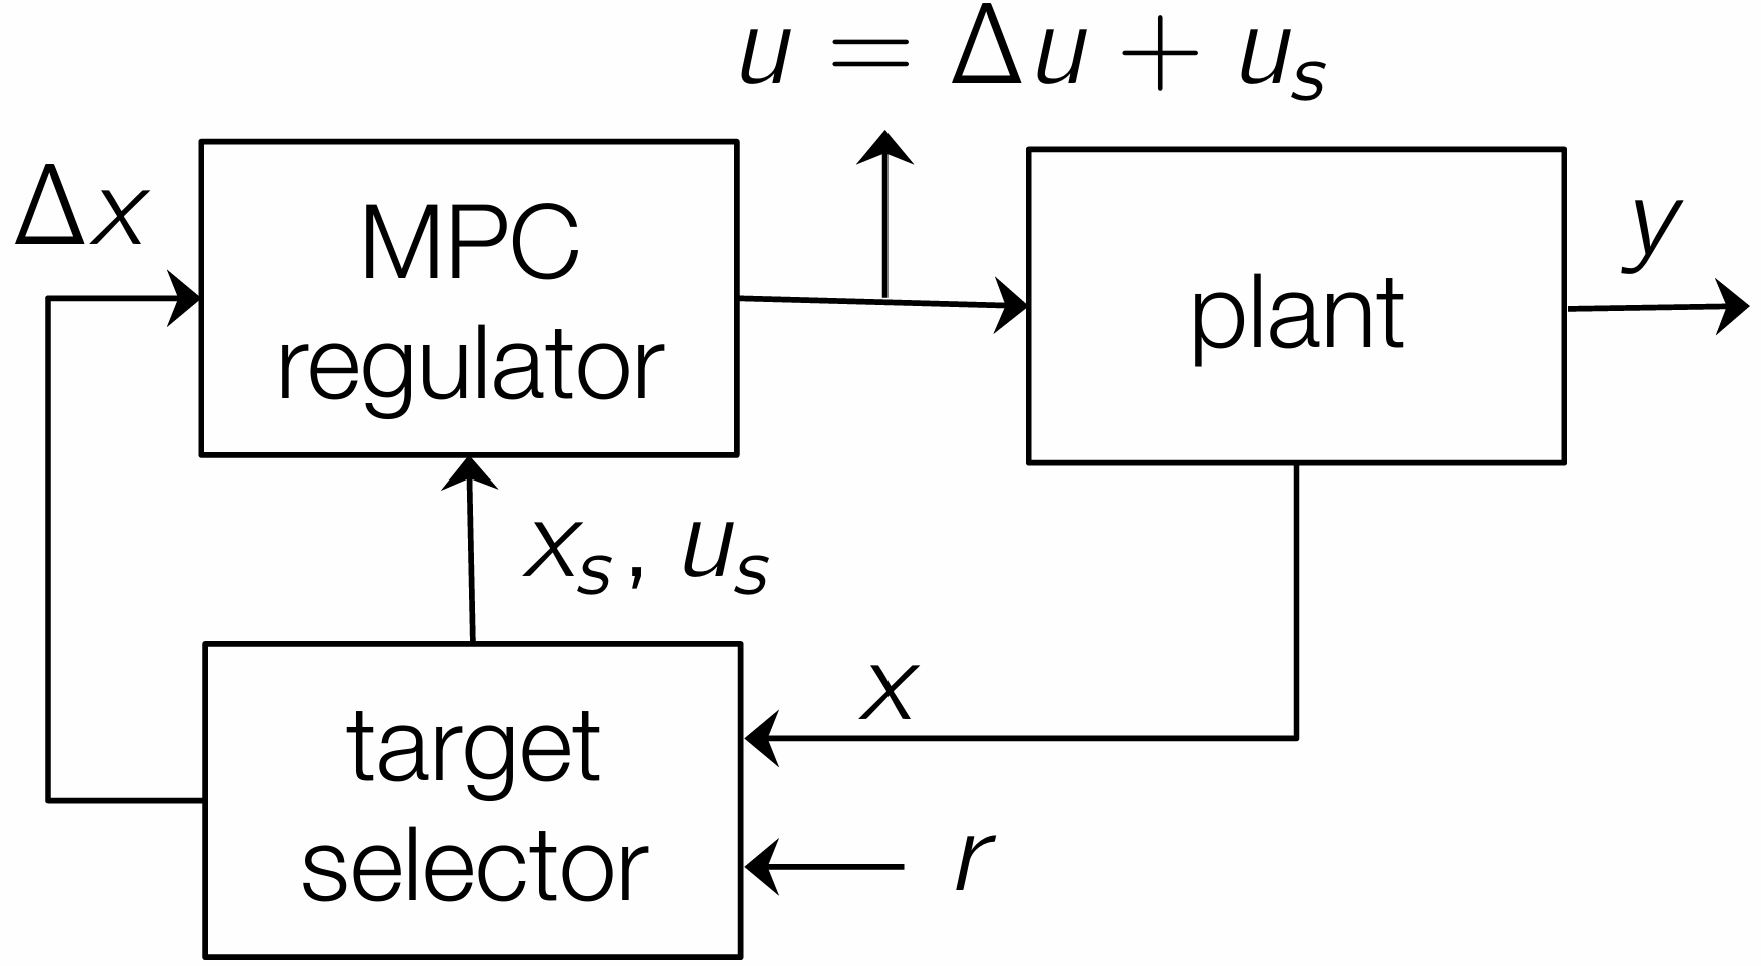
\includegraphics[width=0.9\linewidth]{images/mpc_tracking_diagram.png}
\end{minipage}
\textbf{MPC for tracking: Convergence}\\
Assumption: Feasible target with $x_s\in\mathcal{X}$, $u_s\in\mathcal{U}$ with terminal weight $V_\text{f}$ and constraint $\mathcal{X}_\text{f}$ satisfying:
\begin{itemize}
    \item $(A+BK)x\in\mathcal{X}_\text{f},\;\forall x\in\mathcal{X}_\text{f}$
    \item $V_\text{f}(x(k+1))-V_\text{f}(x(k))\leq-l(x(k)\,,\,Kx(k)),\;\forall x\in\mathcal{X}_\text{f}$
\end{itemize}
IF furthermore the target reference $x_s$, $u_s$ is such that:\\
$x_s\oplus\mathcal{X}_\text{f}\subseteq\mathcal{X}$, $K\Delta x+u_s\in \mathcal{U}$, $\forall \Delta x\in\mathcal{X}_\text{f}$\\
\textcolor{red}{\rightarrow} the cl-system \textcolor{red}{converges to the target reference}\\
$x(k)\rightarrow x_s$, therefore $z(k)=Hx(k)\rightarrow r,\text{ as } k\rightarrow\infty$\\
\textbf{MPC for tracking: Terminal set }\\
Issue: set of feasible targets may be reduced.\\
\rightarrow Enlarge the set of feasible targets by scaling the terminal set for regulation
\begin{itemize}
    \item Scale terminal set by $\alpha$: $\mathcal{X}_\text{f}^{scaled}=\alpha\mathcal{X}_\text{f}$
    \item Thereby invariance is maintained
    \item Choose $\alpha$ s.t. state and input constraints are satisfied (scaling dependent of target)
\end{itemize}
\textbf{Summary: MPC for tracking}\\
\begin{itemize}
    \item Set point tracking problem \Rightarrow Regulation problem after coordinate transformation
    \item If cl-system stable \Rightarrow Set point is achieved
    \item Difficulties:
    \begin{enumerate}
        \item Terminal set is fct. of the target
        \item Ref. change can make the problem infeasible
        \item \textbf{Controller could show offset for unknown model error or disturbances}
    \end{enumerate}
\end{itemize}
\subsubsection{MPC for reference tracking without offset}
\textbf{Constant disturbance acting on the system}:
$x(k+1)=Ax(k)+Bu(k)+B_dd$,\\
$y(k)=Cx(k)+C_dd$\\
\textbf{Goal:} If the system is stabilized in presence of disturbance \\\rightarrow it converges to set point with zero offset\\
Approach in constrained control:
\begin{itemize}
    \item Model the disturbance
    \item Estimate state and disturbance through measurements and models 
    \item Through disturbance estimates find control inputs that remove the offset
\end{itemize}
\textbf{Augmented model}\\
Introduce disturbance model (integral disturbance dynamics)\\
$x_{k+1}=Ax_k+Bu_k+B_dd_k$\\
$d_{k+1}=d_k$\\
$y_k=Cx_k+C_dd_k$\\
Restriction on choice of $B_d,\,C_d$ \rightarrow observability of the augmented model\\
Augmented system is observable iff:
\begin{itemize}
    \item $(A,C)$ is observable
    \item $\begin{bmatrix}
        A-I&B_d\\C&C_d
    \end{bmatrix}$ full column rank ($\text{rank}=n_x+n_d$)\\
    $\rightarrow$ Maximal disturbance dimension $n_d\leq n_y$
\end{itemize}
\textbf{Linear state estimation}\\
State observer for augmented problem\\
$\begin{bmatrix}
    \hat{x}(k+1)\\\hat{d}(k+1)
\end{bmatrix}=\begin{bmatrix}
    A&B_d\\0&I
\end{bmatrix}\begin{bmatrix}
    \hat{x}(k)\\\hat{d}(k)
\end{bmatrix}+\begin{bmatrix}
    B\\0
\end{bmatrix}u(k)+\begin{bmatrix}
    L_x\\L_d
\end{bmatrix}(-y(k)+C\hat{x}(k)+C_d\hat{d}(k))$\\
$\hat{(\cdot)}$\rightarrow estimates of the state and disturbance, $y$ the measured output\\
Error dynamics:\\
$\begin{bmatrix}
    x(k+1)-\hat{x}(k+1)\\
    d(k+1)-\hat{d}(k+1)
\end{bmatrix}=\left(\begin{bmatrix}
    A&B_d\\0&I
\end{bmatrix}+\begin{bmatrix}
    L_x\\L_d
\end{bmatrix}\begin{bmatrix}
    C&C_d
\end{bmatrix}\right)\begin{bmatrix}
    x(k)-\hat{x}(k)\\d(k)-\hat{d}(k)
\end{bmatrix}$\\
\Rightarrow Choose L s.t. error dynamics are asymptotically stable\\


\subsubsection{Offset free tracking}
Lemma: Suppose asymptotically stable observer and $n_y=n_d$\\


\begin{tcolorbox}[eqbox]
\begin{align*}
\text{Observer steady state satisfies: }
\begin{bmatrix}
    A-I&B\\C&0
\end{bmatrix}\begin{bmatrix}
    \hat{x}_\infty\\u_\infty
\end{bmatrix}=\begin{bmatrix}
    -B_d\hat{d}_\infty\\y_\infty-C_d\hat{d}_\infty
\end{bmatrix}
\end{align*}
\end{tcolorbox}

\Rightarrow Observer output tracks measurement $y_\infty$ without offset\\
Goal: Track constant reference $r$: $z(k)=Hy(k)\rightarrow r,\;k\rightarrow\infty$\\
New steady state condition: $\begin{aligned}[t]
    x_s &= Ax_s+Bu_s+B_d\hat{d}_\infty \\
    z_s &= H(Cx_s+C_d\hat{d}_\infty)=r
\end{aligned}$\\
General offset free tracking scheme:
\begin{enumerate}
    \item Estimate state and disturbance $\hat{x},\,\hat{d}$
    \item Obtain $(x_s\,,\,u_s)$ using disturbance estimate
    \item Solve MPC problem using the disturbance estimate $\hat{d}$:\\
    $\min _U\sum_{i=0}^{N-1}(x_i-x_s)^TQ(x_i-x_s)+(u_i-u_s)^TR(u_i-u_s)+V_\text{f}(x_N-x_s)$\\
    subj.to $x_0=\hat{x}(k),\;d_0=\hat{d}(k)$\\
    $x_{i+1}=Ax_i+Bu_i+B_dd_i$\\
    $d_{i+1}=d_i$\\
    $x_i\in\mathcal{X},\,u_i\in\mathcal{U},\,x_N-x_s\in\mathcal{X}_\text{f}$
\end{enumerate}
\begin{minipage}[t]{0.60\linewidth}
\textbf{Summary: offset-free control}\\
Main result: IF
\begin{itemize}
    \item $n_y=n_d$
    \item target steady state problem is feasible
    \item the cl-system converges
\end{itemize}
$\Rightarrow$ Target achieved without offset!
\end{minipage}%
\hfill
\begin{minipage}[t]{0.35\linewidth}
  \centering
  \vspace{-5em}
  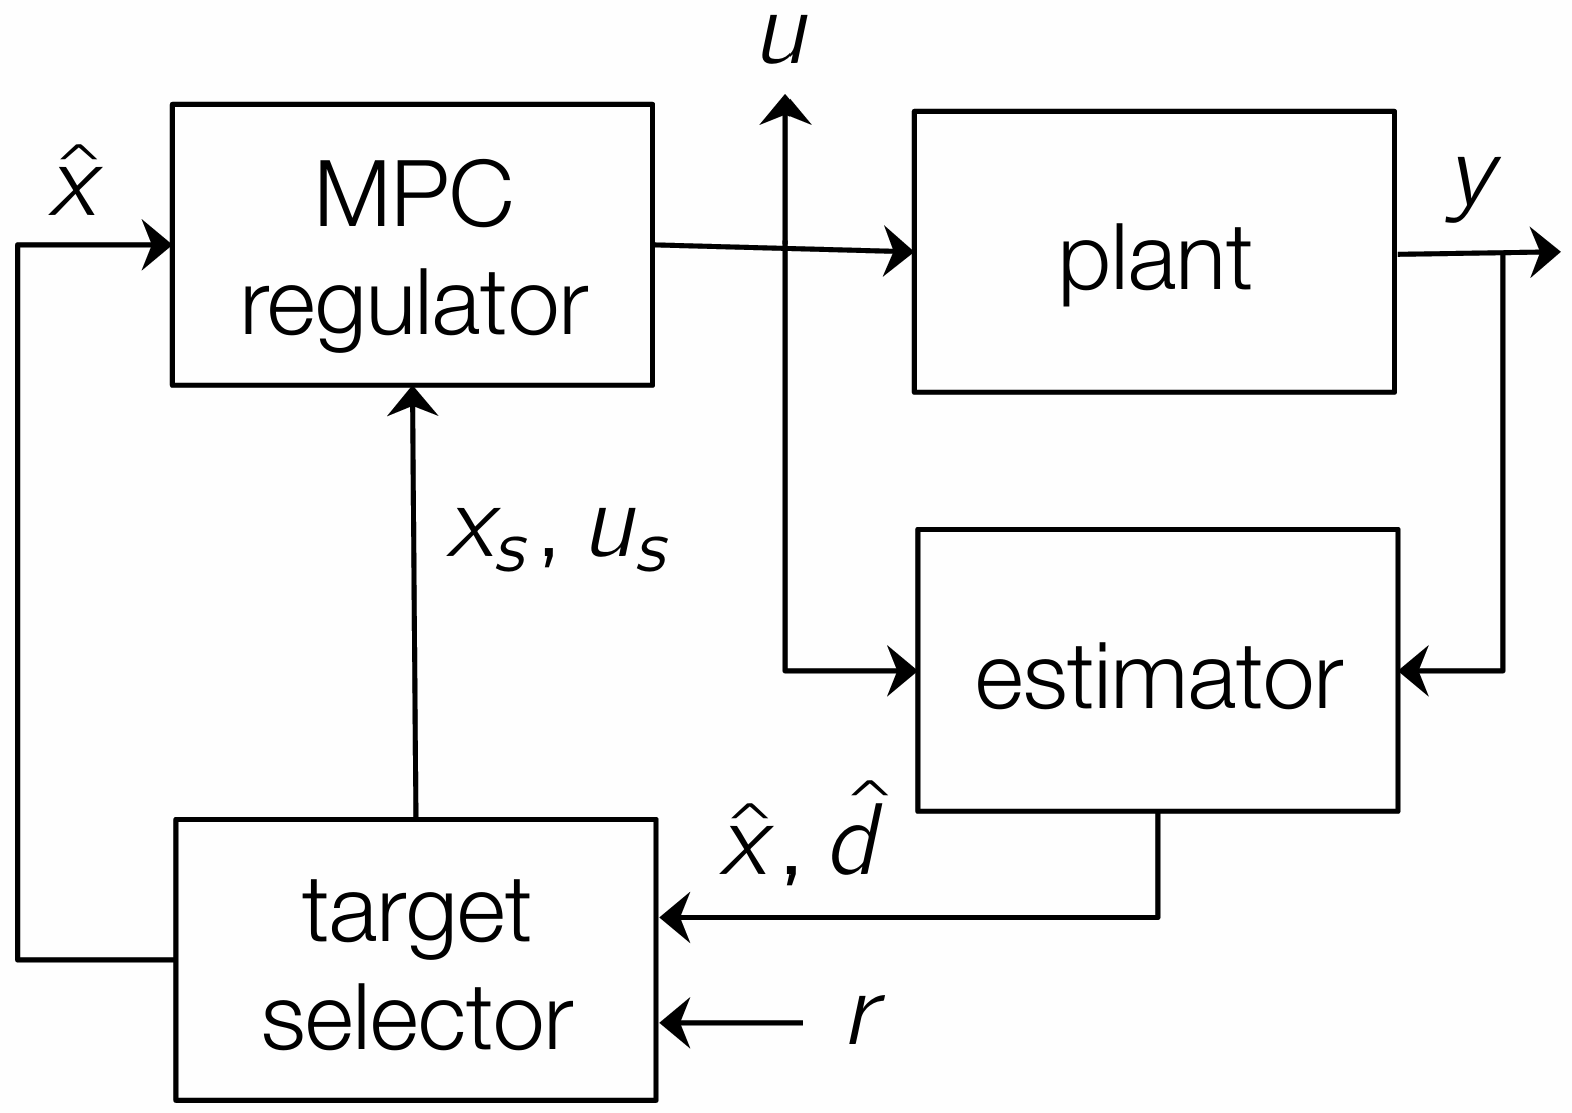
\includegraphics[width=0.9\linewidth]{images/mpc_wo_offset_diagram.png}
\end{minipage}

\subsection{Enlarging the feasible set}
\textbf{Assumptions for Stability of MPC:}\\
\begin{enumerate}
    \item Stage cost is pos. def. (only zero at origin)
    \item Terminal set is \textbf{invariant} under the local control law $\kappa_\text{f}(x_i)$\Rightarrow $x_{i+1}=Ax_i+B\kappa_\text{f}(x_i)\in\mathcal{X}_\text{f},\; \forall x_i\in\mathcal{X}_\text{f}$
    \item Terminal cost continuous Lyapunov function in $\mathcal{X}_\text{f}$ and: $l_\text{f}(x_{i+1})-l_\text{f}(x_i)\leq -l(x_i,\kappa_\text{f}(x_i)),\;\forall x_i\in\mathcal{X}_\text{f}$
\end{enumerate}
\textbf{Important}: Terminal constraint \rightarrow feasible set reduction\\
\textbf{Goal}: MPC without terminal constraint with guaranteed stability\\
\textbf{Note}: Feasible set without terminal constraint is NOT INVARIANT

\subsubsection{MPC without Terminal Set}
    Stability is maintained when removing the terminal constraint if:\\
    1) Initial state in sufficiently small subset of feasible set \;
    2) Horizon $N$ is sufficiently large\\
    \Rightarrow Terminal state satisfies terminal constraint without explicit enforcement in the optimization\\
    \Rightarrow Sol. of finite horizon MPC corresponding to infinite horizon MPC\\
    \textbf{Advantage}: Controller defined in larger feasible set\\
    \textbf{Disadvantage}: Definition of Region of attraction (ROA) or required horizon N difficult \\
    \textbf{Remarks}: Larger horizon length N, ROA \rightarrow maximum control inv. set


    
\subsubsection{Soft constrained MPC}
    Input constraints usually hard vs. State/ output constraints rarely hard\\
    \rightarrow Hard state and output constraints cause complications in the controller implementation
    \Rightarrow In practice: \textbf{State constraints are softened}\\
    \textbf{Objectives}:
\[
\left.
\begin{aligned}
&\text{Minimize violation duration}\\
&\text{Minimize violation size}
\end{aligned}
\right\}
\;\rightarrow\;
\textbf{multi-objective problem}
\]
    \textbf{Soft Constrained MPC problem setup}\\

\begin{tcolorbox}[eqbox]
\begin{align*}
\min_{U,\epsilon}\quad &
\sum_{i=0}^{N-1}\!\left(x_i^\top Qx_i+u_i^\top Ru_i+
\ell_\epsilon(\epsilon_i)\right)
+x_N^\top Px_N+\ell_\epsilon(\epsilon_N)\\[-1mm]
\text{s.t.}\quad &
x_{i+1}=Ax_i+Bu_i,\;
H_xx_i\leq k_x+\epsilon_i,\;
H_uu_i\leq k_u,\;
\epsilon_i\geq0,
\end{align*}
\end{tcolorbox}

    

    \rightarrow State constraints are \textbf{slack variables $\epsilon_i\in\mathbb{R}^p$}\\
    \rightarrow Amount of constraint violation penalized by $l_\epsilon(\epsilon_i)$\\

    \textbf{Original problem}: $\min_zf(z)$\quad
    subj.to $g(z)\leq0$\\
    \textbf{"Softened" problem}: $\min_{z,\epsilon}f(z)+l_\epsilon(\epsilon)$\quad
    subj.to $g(z)\leq \epsilon,\;\epsilon\geq0$\\
    \textbf{Important requirement on $l_\epsilon(\epsilon)$}:
    If original problem has feasible solution $z^*$\\\rightarrow the softened problem should have the same solution $z^*$, and $\epsilon=0$\\
    \textbf{Issue:} E.g. $l_\epsilon(\epsilon)=s\cdot\epsilon^2$ doesn't satisfy this requirement for any $s>0$\\
    \textbf{Main result: Exact Penalty function}\\
    $l_\epsilon(\epsilon)=\nu\cdot\epsilon$ satisfies the requirement for any $\nu>\lambda^*\geq0$ \\($\lambda^*$ is the optimal Lagrange multiplier of teh original problem)\\
    Extension to multiple constraints $g_j(z)\leq0,\,j=1\,,\,...\,,\,r$\\
    $l_\epsilon(\epsilon)=\nu\cdot||\epsilon||_{1/\infty}+\epsilon^TS\epsilon$ ($\nu>||\lambda^*||_D$ and $S\succ0$\rightarrow used to weight violations differently, $||\cdot||_D$: dual of the chosen norm)\\
    \textbf{Properties of the quadratic penalty:}\\
    \rightarrow Increasing $S$ causes \textbf{hardening of the soft constraints} (reduced size of violation BUT longer duration)\\
    \rightarrow $\nu$ large enough: satisfaction of constraints if possible (large $\nu$: increased peak violations and decreasing duration)\rightarrow \textbf{better to keep $\nu$ as small as possible}\\
    \textbf{Summary: Soft constraints}:\\
    \rightarrow Soft constraints recover feasibility when constraints cannot be satisfied\\
    \rightarrow Allow for \textbf{tradeoff btw. violation duration vs. size} \\
    \rightarrow Good closed loop properties  (standard methods of softconstrained MPC: no stability guarantees for unstable ol-systems)\\
    \rightarrow \textbf{Separation of Objectives}: Solve two optimization 1) Min. violation 2) Optimize performance (Simpler to tune but require two optimizations)